\documentclass[../report.tex]{subfiles}
\begin{document}	
	
\chapter{Introduction} 
Communication and collected thinking is the key to the development and continuous evolution of human civilization which is driven by data - “The new oil of this digital era”. With the advent of \gls{iot}, it has been estimated that by 2020 there will be 26 billion connected devices \cite{gartner_iot} and all that can be connected will be connected. Today only about 40 percent \cite{internet_users} of the world’s population use the Internet and the amount of data produced per minute through different social media platform like Facebook, Youtube, Twitter, Flickr, Instagram, Linkedin, Blogger, Whatsapp etc. is already growing exponentially. 

\begin{figure}[h]
	\centering
	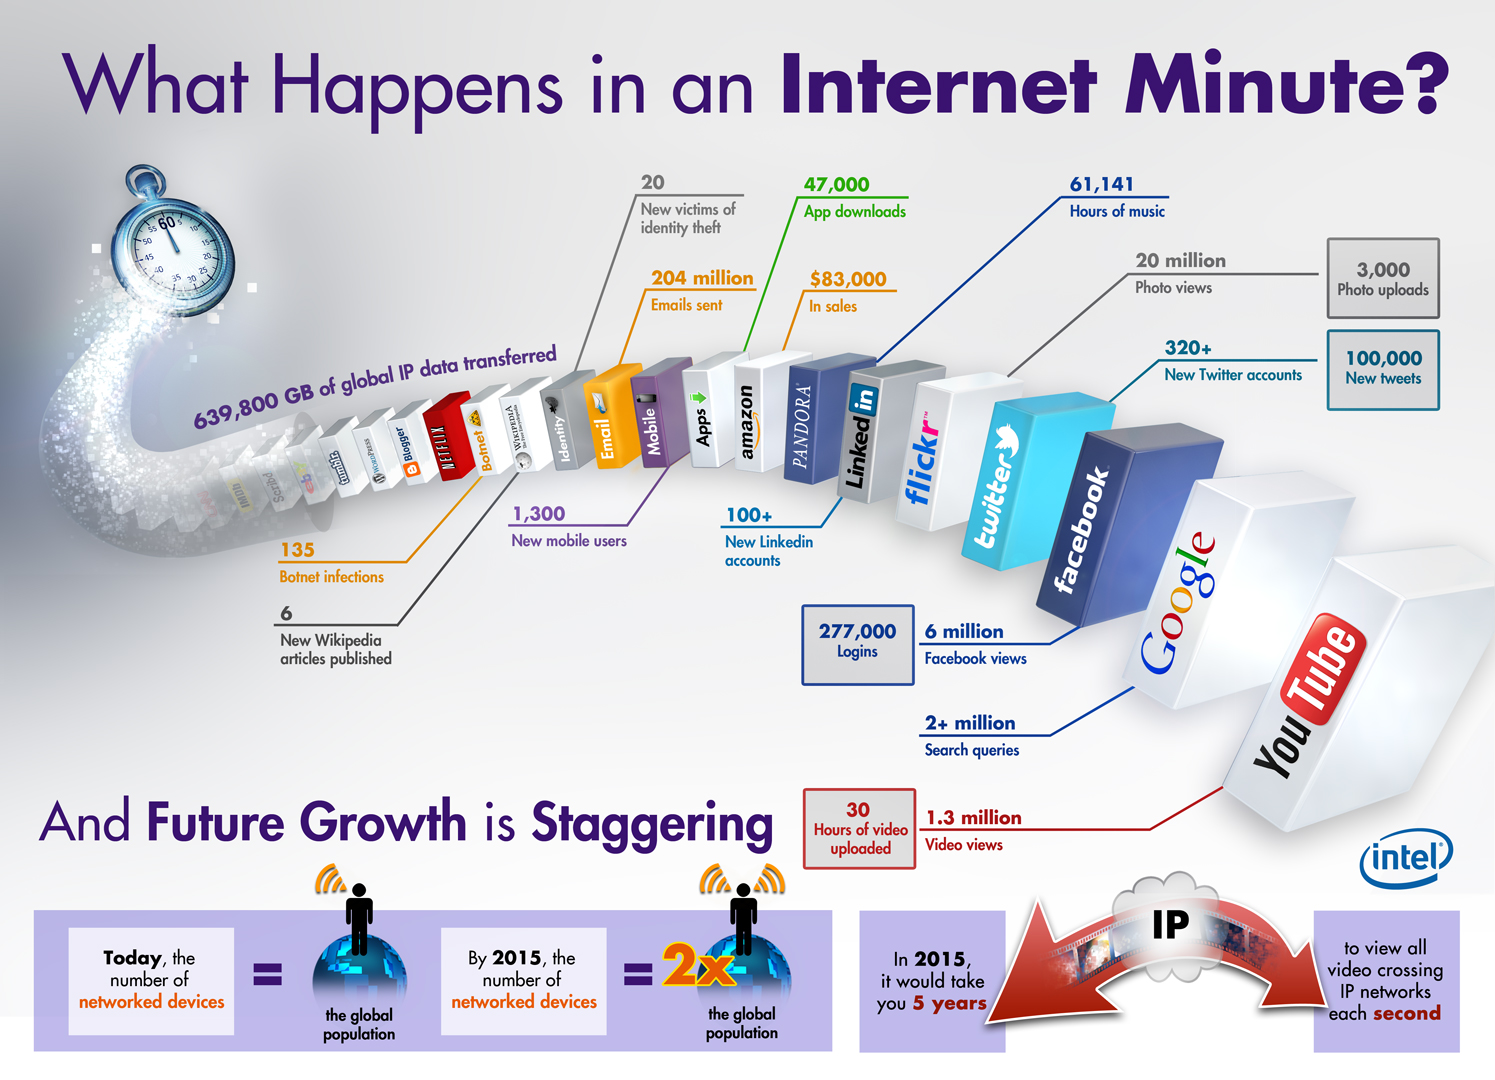
\includegraphics[width=0.75\textwidth]{1-Internet-minute}
	\caption{What happens on internet per minute \cite{internet_minute}}
	\label{fig:1_internet_minute}
\end{figure}
\todo{Edit this picture}
\noindent Eventually, with the inclusion of world's population into the cyberspace world this data growth will be more than ever. \par

Also, with the advent of mobile communications, there has been a huge surge in the voice as well as data traffic all over the world. It has been estimated in Ericsson's mobility report \cite{ericsson_mobility_report} that 70 percent of world's population will use smart-phones by 2020 and 90 percent of the world's population over 6 years old will have a mobile phone by 2020. 

\begin{figure}[!tbp] %h
	\begin{subfigure}[t]{0.45\textwidth}
		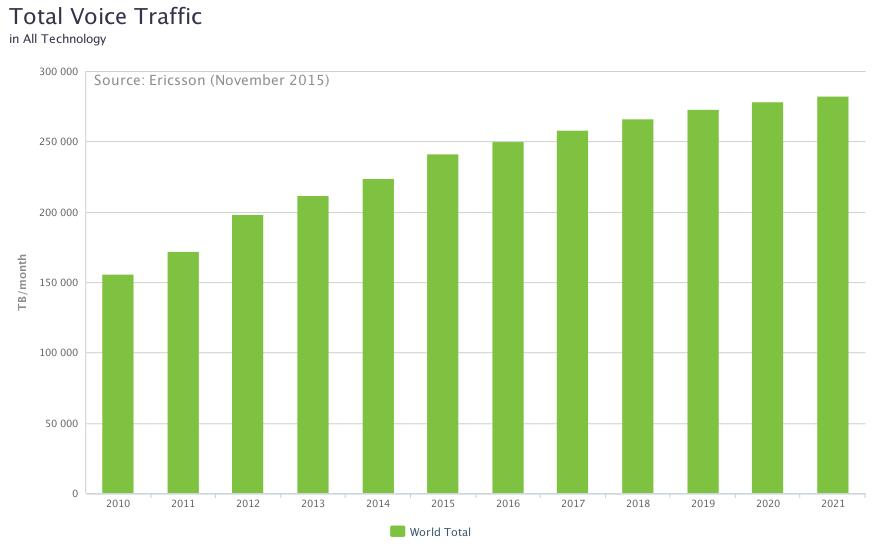
\includegraphics[width=\textwidth]{1-voice-traffic-forecast}
		\caption{Voice data traffic forecast all over the world}
		\label{fig:1_voice_traffic_forecast}
	\end{subfigure}
	\hfill
	\begin{subfigure}[t]{0.45\textwidth}
		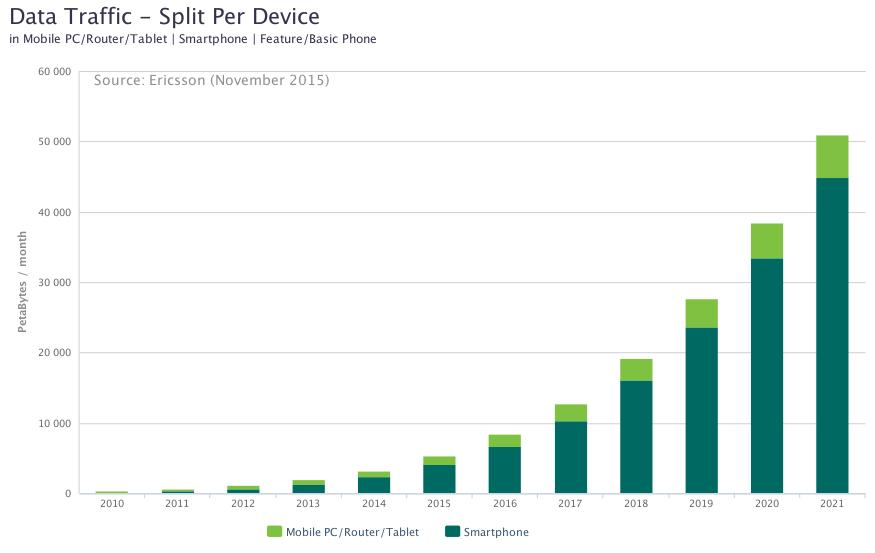
\includegraphics[width=\textwidth]{1-data-traffic-forecast}
		\caption{Data traffic forecast for different devices}
		\label{fig:1_data_traffic_forecast}
	\end{subfigure}
	\caption{Voice and data traffic growth forecast by 2020 as per Ericsson, generated using \cite{ericsson_traffic_exploration}}
\end{figure}

Currently, the telecommunications industry is moving towards \gls{ims} core networks which is a transition towards full IP based networks. So how is this humongous traffic managed? The answer is the optical fiber, which serves as the backbone of all the communication systems. The performance of optical fiber network is unprecedented and it is this backbone which gives us an unfathomable user experience. The current internet architecture has already pushed the optical fiber to the network edges and the trend is to push it as closer to the processor as possible. This has already opened up a new area of “Siliconizing photonics” based on the decades of research obtained from microelectronics industry. The electronics industry have pushed the boundaries of the processing speed of \gls{ic} after the invention of semiconductors and are currently at the edge where Moore’s Law is at its upper limit. Although, with the current technology we have a decent processing power but what about the interconnects between the \gls{ic}. Transmission of signals through copper interconnects would definitely slow things down. Think of a data center processing peta-bytes of data per minute, where interconnects between processors can add up to a significant delay. These losses can be overcome by adding optical interconnects using the current technology which can also operate at low power and better efficiency catering to the needs of the environment.
	
	\section{Motivation}
The movement of data in a computer is almost the equivalent of movement of traffic in a city, where data flows fast in the congested microprocessor but is delayed in the interconnects. Intel processor speed and bus speed comparison \cite{intel_proc_compare} shows that although we have achieved good processing speed, the interconnects always find difficulty in catching up with the processing speed. Obviously, the closer engineers can bring the optical superhighway to the microprocessor, the fewer copper bottlenecks can occur. Until recently, exponential increases in the speed, efficiency, and processing power of conventional electronic devices were achieved largely through the downscaling and clustering of components on a chip. However, this trend toward miniaturization has yielded unwanted effects in the form of significant increases in noise, power consumption, signal propagation delay and aggravates already to serious thermal management problems. Alternatively, the wires can be made fatter, but then you'll run out of space and the packing density will be inefficient.  As a result, traditional microelectronics will soon fall short of meeting market needs, inhibited by the thermal and bandwidth bottlenecks inherent in copper wiring. Photons don't suffer from these limitations; their biggest problems are absorption and attenuation, neither of which is an issue over the distances inside a computer, or even across a room. Today Silicon Photonics \cite{silicon_photonics} Technology is a new approach to make optical devices out of silicon and use light (photons) to move huge amounts of data at very high speeds with extremely low power over a thin optical fiber rather than using electrical signals over a copper wire. Since, already enough capital investments has been done on perfecting the current fabrication technology and infrastructure, engineers are working on creating monolithic design of integrated circuits which use light in place of electric signals. Organizations are trying to bridge this gap by creating highly integrated photonic and electronic components that combine the functionality of conventional \gls{cmos} circuits with the significantly enhanced system performance of photonic solutions. By allowing for the seamless integration of optical and electronic components on silicon-based substrates, this technology holds the key to fulfilling market needs for higher bandwidth and processing speed at lower power and cost.\par

Silicon Photonics is an emerging market and researchers are actively working on creating monolithic \gls{ic} design with optical components to cope up with the future demands \cite{optical_linking}. Researchers are coming up with new avenues indicating that fiber information capacity can be notably increased over previous estimates \cite{temprana_overcoming_2015} which can double fiber optic capacity. The silicon photonics market is estimated to grow to 700 million USD by 2024 \cite{silicon_photonics_growth_2015} with a \gls{cagr} of 38 percent. Photonic devices made on \gls{soi} platform is compatible with \gls{cmos} electrical circuits since they are based on same material. It is also promising in developing on-chip integration for telecommunications applications and servers in data centers \cite{jalali_silicon_2006}. Various kinds of silicon photonic devices like switches \cite{wu_mems-enabled_2015,nikolova_scaling_2015,lu_low-power_2014}, modulators \cite{dong_silicon_2015,chen_generation_2013}, photodetectors \cite{urino_demonstration_2012,chang_high-power_2015}, delay lines \cite{garcia_design_2015,mattarei_variable_2014}, sensors \cite{janz_silicon_2007,lim_laser_2010,ryckeboer_glucose_2014} etc. have been reported till date. All these things have corroborated interest into silicon photonics which are based on \gls{soi} platform.\par   

However, these photonic devices based on \gls{soi} waveguides are sensitive to polarization due to large structural birefringence, which might induce \gls{pdl}, \gls{pmd}, and \gls{pdw} limiting their usability. To overcome these challenges \gls{pr} are engineered on \gls{soi} for \gls{oeic} and various designs have already been demonstrated \cite{xie_efficient_2015,velasco_ultracompact_2012,leung_numerical_2011,wang_design_2014,dai_novel_2011,wirth_efficient_2012,chen_compact_2011} which will be discussed in later sections. The main principle of these proposed solutions are based on varying \gls{ri} by introducing asymmetry in the waveguide structure which is not tunable. Also, in some cases the designs \cite{sarmiento-merenguel_demonstration_2015}, if used in commercial applications for miniature interconnects, would incur inefficient packing density since too much space is required to achieve high and robust tuning. Apart from that there might also be thermo-optic induction problem which might change phase of the wave in other waveguides in high compact density environment as silicon is highly susceptible to thermal changes \cite{ibrahim_athermal_2012}. Also, \gls{tpr} have been reported which works on the principle of Berry’s phase, a quantum-mechanical phenomenon of purely topological origin \cite{xu_electrically_2014}. But, since the design is based on out of plane waveguides it might be difficult to achieve efficient mass production without a complex manufacturing process. The general goal of the thesis work is to realize efficient \gls{tpr} using \gls{mems}, to achieve improvement over the current available research solutions, to cater needs of the future industry.    
	\section{Objectives}
The current situation landscape in Silicon Photonics is quite exciting and a number of problems are there in the industry to realize a final optimal and robust prototype. The main objective of this thesis work is to design and fabricate low power \gls{tpr} which can primarily mitigate the drawbacks discussed earlier. To tune at sufficient low power, \gls{mems}. The waveguides will be build upon current Silicon fabrication technology which will be characterized using an automated measurement setup to minimize coupling loss using grating couplers. In this thesis following objectives will be addressed:
\begin{itemize}
	\item[$\square$] How to design a \gls{mems} tunable polarization rotator?
	\item[$\square$] How to simulate the design using \gls{mems} techniques like Comsol, CST etc.?
	\item[$\square$] How to effectively characterize the system with the measurements available?
	\item[$\square$] By how much can the power consumption be reduced in comparison to current state of the art?
	\item[$\square$] What is the \gls{per} that can be achieved through redesign?
	\item[$\square$] What packing density can be achieved through this design in comparison to the available solution for \gls{oeic}?
	\item[$\square$] How easily can the design be fabricated?
	\item[$\square$] Efficiency of the fabricated device?
\end{itemize}

	\section{MEMS and silicon photonics}
\gls{mems} are micrometre-sized sensors and actuators that are used in many devices in our everyday life (eg. Gyrometer and accelerometer in our smartphones). Using the same fabrication technology, one can fabricate on-chip optical circuits, which drastically improve the performance of telecommunication systems. However, both \gls{mems} and silicon waveguides have been independently developed. This project aims to bring together both fields to try out new ideas to enable new applications and to improve existing ones. 
	
	\section{Importance of these systems}
Silicon photonics is on the verge of creating a newer technology trend. It is on the brink of creating a technological revolution where semiconductor industry stood back 60 years from now just before the discovery of transistors. If this technology is developed successfully it can keep up with the tremendous data processing power needed by the current networking servers to deliver services. Since use of optics can also increase the bandwidth in a many-fold manner it can cater the needs of data rate needed by the futuristic networks. Also, as the vision is to move everything closer to the chip this technology can deliver \gls{ic} which can be easily fit into futuristic devices. Using \gls{mems} for the tuning will ensure high resolution at very low standing power. This is also important because light transmitted to an optical circuit will typically come from an optical fibre, and optical fibres emit light with random polarization. Theses systems can expand the boundary of optical networks and bring it closer to the end devices by transgressing the network edges where optical fibers are currently located.
	
	\section{Outline of this thesis}
The outline of the thesis is as follows: Background, motivation and the research questions being addressed, is discussed in Chapter 1. In Chapter 2, the current state of art for the available solution is discussed along with the background literature required. Here, also the working principle of the current available design are explained along with the areas which can be improved. Chapter 3 discusses about the design of the final system and the results obtained about the simulation setup. In Chapter 4, documentation about the fabricated design is provided along with currently available standard fabrication technologies. Results and characterization are an important part of the work, which is discussed in Chapter 5. Finally, Chapter 6 and 7 discusses about the conclusion and future work possibilities respectively along with the known limitations of the system if any.  
	
\end{document}
